\documentclass[]{interim_report}
\usepackage{graphicx}
\usepackage{hyperref}


%%%%%%%%%%%%%%%%%%%%%%
%%% Input project details
\def\studentname{Eva Darulov\'{a}}
\def\projecttitle{BON Software Model Consistency Checker for Eclipse}
\def\supervisorname{Dr. Joseph Kiniry}
\def\moderatorname{Dr. Barry Smith}


\begin{document}

\maketitle
\tableofcontents\pdfbookmark[0]{Table of Contents}{toc}\newpage

%%%%%%%%%%%%%%%%%%%%%%
%%% Your Abstract here
\begin{abstract}
Modelling languages specifying a system independently from its implementation are particularly useful during analysis and design stages of a system. An implementation-specific formal language translates those requirements directly into code, annotations and possibly assertions. Both approaches have their advantages and should ideally be used hand in hand. In practice however, mostly due to lack of tool support, the model of a project will not be updated once a formal specification is in place, thus rendering it useless. This project interlinks the BON and JML modelling languages by creating a mapping between their structure and assertion features and by providing tool support for consistency 
checking. 

\end{abstract}
\newpage

%%%%%%%%%%%%%%%%%%%%%%
%%% Acknowledgments

%\chapter*{Acknowledgments}

%In your Acknowledgments section, give credit to all the people who helped you in your project.

%%%%%%%%%%%%%%%%%%%%%%
%%% Introduction
\chapter{Introduction}
%%%%%%%%%%%%%%%%%%%%%%
%%% Project Specification
\section{Project Specification}
Business Object Notation (BON) has been developed for designing and analysing object-oriented programs. It is designed to enable a seamless and reversible development process as well as software contracting. It provides a textual, graphical and an informal representation of the system to be developed. Thus it can close the communication gap between technical and non-technical people (e.g. programmer and project manager) involved in the design and implementation of software.

The Java Modeling Language (JML) is a formal specification language for Java. It follows the Java syntax closely and its annotations are inserted directly into code. By doing so, it is easy for developers to learn and convenient to apply. It employs the design by contract approach by specifying preconditions, postconditions and invariants. With its extensive tool support it is greatly suitable for development of commercial software.

To make the most of a software model it has to be used throughout the development process, not just for the initial draft. For example, it can be used to update high-level manager on possible changes in the implementation without confusing them with technical details. This can only be achieved when the model is always up-to-date during whole of the development process. This project aims to provide such synchronisation by checking the consistency between a BON model and the corresponding Java source code with JML annotations.

Mandatory: 
\begin{itemize}
\item Familiarisation with software modeling and the BON method/language
\item Familiarisation with design by contract and the Java Modeling Language (JML)
\item Familiarisation with development of Eclipse plugins
\item Create a mapping between BON features and JML features and identify possible issues where the two notations may not be (fully) compatible
\item Implement an Eclipse plugin that reads in a BON file (format to be decided) and highlights differences in the corresponding Java/JML souce code
\item Design and implement a test program 
\end{itemize}
 
Discretionary: 
\begin{itemize}
\item Design a GUI that is clearly arranged and flexible
\item Include the option to generate Java skeleton code with JML annotations from BON model
\item Make checks possible in both directions (BON - Java and Java - BON)
\item Internationalize the plugin
\item Make the plugin effective (e.g. it will only check lines of code that have changed since the last check)
\item Allow for JML and BON to be extendable (e.g. custom tags, keywords)
\end{itemize}
 
Exceptional: 
\begin{itemize}
\item Write, submit, and publish a paper on the results   
\end{itemize}
 
 %%%%%%%%%%%%%%%%%%%%%%
%%% Purpose of Project
\section{Overview}
The purpose of this project is to combine a modelling method with an implementation and specification language. The result provides a seamless software engineering process from initial design and analysis stages to implementation, testing and possibly verification. Object oriented (OO) programming has proven to be popular and most importantly suitable for many of today's software projects. Another related emerging approach is Design by Contract (DbC)~\cite{MEYER:1992}. It expresses the responsibilities and guarantees of each class and provides thus a way to make statements about the reliability of a software system~\cite{MEYER:1997}. However, this second approach is not as widely used in software development. By choosing and combining a modelling language and an implementation language that use both of these approaches, but are relatively easy to learn, and by providing an example tool support for their integration, this project hopes to promote the use formal specifications and to help building more reliable software.\\
The Business Object Notation (BON)~\cite{WALDEN:1995} is the modelling language of choice, because it provides both a method and a (graphical) notation. The object oriented paradigm and DbC are directly supported by its structure and its assertion language. In contrast to other modelling languages, it is also simple and compact and can be easily learned~\cite{PAIGE:1999}.
The implementation language of choice is Java~\cite{GOSLING:2005} for it is widely used, accepted and object oriented. However, since by itself it lacks a specification language to enforce DbC, the Java Modelling Language (JML)~\cite{LEAVENS:2008}~\cite{LEAVENS:2006}  has to be included. It can provide a complete formal specification of the system and due to its increasing popularity various static checking and verification tools are available~\cite{BURDY:2005}.
A plugin for the popular Eclipse IDE that checks the consistency between a BON model and its Java implementation will demonstrate how these two languages can be used hand in hand. \\
BON and Java with JML are all object oriented languages, hence they are reasonably similar for combining them in one software engineering process. However, since they developed independently, their syntax and semantics are expected to differ in places. These conflicts have to be identified and either resolved automatically (by extending or adapting the languages) or marked otherwise so that they can be reviewed manually.\\
Chapter 2 describes some important and relevant details of the BON, Java and JML languages and chapter 3 gives an overview about the progress of the project so far and a short example of such a mapping.



\chapter{Background Research}
%% This section provides details about the elements used in the project: Design by Contract, BON, Java, JML and Eclipse IDE plugin development.

%%%%%%%%%%%%%%%%%%%%%%
%%% BON Background
\section{BON - a modelling method}
BON~\cite{WALDEN:1995} is a modelling method for design and analysis of object oriented systems, where a system means a set of classes that constitute a computer program. It intends to put into practice the core of the object oriented paradigm. The main ideas here are seamlessness (the same model can be used from design to implementation stages), reversibility (one can turn design into code but also code into a high-level description) and software contracting. Especially the last point is becoming increasingly important when trying to build reliable software. In this approach called \emph{Design by Contract}~\cite{MEYER:1992}, a 'contract' is set up between a \emph{client} (a class) that uses the services of a \emph{supplier}  (a function of another class). It specifies the minimum requirements the client has to obey before he can call a function (the \emph{precondition}) and it specifies the minimum that the supplier guarantees to return (the \emph{postcondition}). Additionally, each class should specify an \emph{invariant} - essentially a set  of predicates that have to hold true at any point in time.\\
BON specifies both a notation as well as a process for OO systems. Here, only the model notation will be investigated but details about the process can be found in~\cite{WALDEN:1995}.
There are three basic ways to describe the system. An informal description provides a very high-level overview of the structure, mostly in plain English. A static model, gives a detailed description of the structure, and finally a dynamic model describes the functionality.
Only the formal description is considered in this case since it most closely corresponds to implemented source code.\\
The initial definition of the syntax and semantics~\cite{WALDEN:1995} has been intentionally kept as simple as possible while containing the most important object oriented concepts. It is explicitly meant for extension and adaptation to a particular context, implementation language or available tools. Presented here are the features of particular interest to this project.\\
The basic element of the formal description is the class. Since BON is strongly typed, each class also represents a type. Each class consists of a name, a header, an inheritance clause, a set of features (corresponding to Java methods) and an invariant. 
The name is unique in the system and serves thus as an unambiguous identifier. 
Class header (see table 2.1) convey more detailed information about the intended use of the class ~\cite{WALDEN:1995}.
%%Class header table
\begin{table}[h]
\begin{footnotesize}
\begin{tabular*}{1.0\textwidth}{@{\extracolsep{\fill}}@{}l | @{}l}
deferred & class not (fully) implemented and meant for inheritance\\
effective & class is implementing a deferred class or reimplementing an interface\\
root & a process can start from here. There must be exactly one root class in each system~\cite{PAIGE:2000}.\\
interfaced & all features are visible for everyone\\
reused & class is reused from a library\\
persistent & class instances are potentially persistent\\
generic & class is parametrized. The allowed types can be further constraint.\\
\end{tabular*}
\end{footnotesize}
\caption{\label{fig:logo} Class header}
\end{table}%
%One can see that the semantic meaning is not set in stone and open for interpretations, as the cases of root and interfaced keywords illustrate.\\
Any class providing some sort of functionality also has a set of features. Each feature has a class-unique name, return and parameter types, a renaming clause and a pre- and postcondition. 
Additionally, one may define a feature as deferred (not implemented), redefined (inherited from a parent class with a changed implementation) or effective (implemented) which is also assumed when no such modifier is given.
Inherited features that are being redefined can also change their name in the process and this change is stored in a renaming clause.
Features may also specify their visibility. If the feature clause is supplemented by a list of class names, only objects of this type are allowed access to the features listed within. Default or not specified visibility is the equivalent to Java's public modifier and stating NONE as the only class allowed is the equivalent to private. This also specifies the visibility of features for specification purposes.\\
BON categorises features into two types: queries and commands. While the first returns some value, but does not change the state of an object, the latter does not return anything but may change state. This distinction is important, as only queries may be used in assertions, as no side-effects are allowed here. Thus all constraints are written using queries and BON's assertion language~\cite{WALDEN:1995}. Invariants, preconditions and postconditions are inherited by all child classes and must be obeyed. When redefining features, preconditions may only be weakend, and postconditions strenghtened as prescribed by DbC~\cite{MEYER:1992}. In addition, the covariant rule for feature signatures applies to ensure correct and sensible use of inheritance relations.\\
Except for the name of a class or a feature, all elements are optional. Therefore providing default values for omitted elements becomes an important part of describing a notation. In the case of preconditions, postconditions and invariants, these are assumed true by default to ensure consistency of the whole model~\cite{MEYER:1992}.\\
Apart from inheritance, classes can be related by two other types of client relations. There is an association between a client and a supplier when the client \emph{uses} the services of the supplier and there is an aggregation relationship if the supplier class is an inherent and fundamental \emph{part} of the client. There exist different types of client relations and also with different multiplicity. These are still being studied as part of the EBON (Extended BON) project~\cite{EBON:2008}. Thus the most simplest forms of associations and aggregations is assumed.\\
BON also provides a way of compressing class charts by means of clusters. Classes are grouped into clusters on which one can define client relations, which may apply to all or only to some classes in the cluster, however the exact semantics are still being developed. Since they ultimately can be expanded into class relations only, we will only look at fully expanded static charts with classes only.\\ 

%%%%%%%%%%%%%%%%%%%%%%
%%% Java
\section{Java - an object oriented programming language}
Java is a general-purpose programming language introduced in~\cite{GOSLING:2005}. It has gone through several revisions and substantial changes have been introduced in Java 5.0, hence this version will be taken as the basis for this project. Here only elements of particular interest are presented, for an introduction see~\cite{HORSTMANN:2007}.\\
Java is strongly typed, with primitive and reference types, with the latter further divided into class, interface and array types~\cite{GOSLING:2005}. In comparison, all types in BON are class types with no fixed set of basic types; these are meant to be user defined. As far as typing is concerned interfaces can be used as class types and can be used to emulate multiple inheritance, since unlike BON inheritance is restricted to one parent class only. The implementation details differ since an interface can only contain implicitly public static final fields and implicitly public abstract members, so that particular care has to be taken with respect to consequences of these restrictions.\\
A class or interface API consists of a set of modifiers, generic parameters, an inheritance clause, an interface clause, a constructor and a set of members (fields, methods, member classes). A method's API consists of a set of modifiers, a return type, a set of parameters and an exceptions clause. Most elements are optional; one only needs to specify whether a type is a class or an interface and a name to make the compiler happy. Classes are compartmentalised into packages and the rule applies that class names only have to be package unique, so that they are being identified by their fully resolved name which includes the package hierarchy as well. Hence, it is clear that Java packages and BON clusters are related only partially. Also unlike BON, Java allows duplicate method names through method overloading so that methods are identified my their name and signature, but does not allow renaming of methods. One should also note that the original BON model does not feature the concept of a constructor. \\  
Java fields can also be thought of as methods with no formal parameters that return the value of some (hidden) variable. By close inspection one can see that no information is lost by this point of view. Since BON does not have a separate notion for attributes this presumption will be made throughout. Java does not make a distinction between a query-like or command-like method, so that in general methods will be a mixture of the two. Only in the case of fields, one can clearly see that they are queries, since they cannot change the state of an object.\\
Java defines four types of visibility: public, protected, default (package-private) and private. The visibility in BON is only bound to specific classes and not clusters or other concepts, so that protected and package-private visibility does not have a direct equivalent in the model. \\
Since Java 5.0, the covariant rule with overriding applies, but to return types only so that there may be a discrepancy between the formal parameters of the implementation and the BON model as the covariant  rule here applies to parameters as well.\\ 
A special feature of Java are exceptions, which will be thrown when semantic constraints are violated or when thrown explicitly by the programmer. They are a means for error handling that is meant to be robust and disallowing for unpredictable behaviour~\cite{GOSLING:2005}. Ideally, with the use of DbC, these violations should not occur. Exceptions will be considered an implementation detail, since the BON software model only describes the correct use of classes and leaves out details about consequences of violations.\\


%%%%%%%%%%%%%%%%%%%%%%
%%% JML
\section{JML - a specification language}
JML is a specification language tailored for Java~\cite{LEAVENS:2006}. It is particularly accessible, even for beginners, since it mostly uses an extended Java syntax and can be included directly in Java source code in form of annotation comments or alternatively in separate files. It describes the interface and the behaviour of Java elements and is thus a behavioural specification language.  Here the extensions of particular interest in the context of a mapping to the BON software model are presented, while disregarding implementation details particular to Java. JML defines several language levels~\cite{LEAVENS:2008} which categorise its features according to their (tool) support. Levels 0 and 1 contain features that should be supported by most tools and that are also most widely used, hence these will be the ones under consideration here.\\
JML defines the interface and the behaviour of a Java module, such as a class or a method, by extending the interface with a specification. The interface is the standard Java declaration (in case of a method this is the method declaration) and the behaviour is specified by an annotation comment. This can be given in a light-weight or a heavy-weight form. The former only supplies the minimal information needed or wanted, whereas the latter is intended to supply a full specification. Both give the specification by means of several clauses, with the main difference being that different assumptions are made when a particular clause is omitted. Light-weight omissions are mostly regarded as not specified, where the specific value is tool dependent and has to be decided based on the context. In the heavy-weight case the value will follow the definition of DbC, for example true for preconditions. Heavy-weight specifications are further subdivided into normal-behaviour and exceptional-behaviour cases. However, this is only syntactic sugar and can be expanded into a standard specification~\cite{RAGHAVAN:2005}. Thus using the correct default values, every specification can be written as a complete specification.\\
A full specification of a class includes an invariant and a specification for each method, which includes the following clauses (language level 0 and 1 only)~\cite{LEAVENS:2008}:
\begin{itemize}
\item precondition
\item frame conditions 
\item postcondition 
\item signals-clause, signals-only-clause which specifies exceptions
\end{itemize}
Frame conditions specify which locations (fields or local variables) may be changed during the methods execution. These must include all locations, even those that are being changed temporarily or are not observable by the client.
These clauses can be given in several parts, however since BON only allows a single clause, it is more convenient to (automatically) join all parts. This applies also to invariant constraints, which may be distributed throughout the class body. As in BON, all specifications are inherited and must be obeyed. \\
JML extends the Java syntax by operators and expressions to allow for the specifications to be written in form of predicates, including set operations and quantifiers. Other commonly used expressions are (for a complete list see~\cite{LEAVENS:2008}):
\begin{itemize}
\item {\tt pure} - marks a method or a constructor as side-effect free, that is no locations are being assigned to. This effectively classifies the method as a query, thus it may be used in assertions.
\item {\tt old} - refers to a variable's value before the methods execution. 
\item {\tt result} - refers to the return value of the method.
\item {\tt for\_all} and {\tt exists} - universal and existential quantifier
\item {\tt non\_null} and {\tt nullable} - all references are by default non-null. If null is allowed as a valid value, this has to be explicitly specified. 
\end{itemize}
All specifications obey the same visibility rules as the members they apply to. It is therefore not permitted to use a private field inside a public specification. If an inaccessible field or method is needed though, it can either be marked as {\tt spec\_public} or {\tt spec\_protected}, which changes the visibility for specifications. Or one can introduce a model field or model method that abstracts the field or method for specifications only so that it will not be part of the program itself. This approach is commonly used when specifying interfaces, since they may only have constant fields.\\
Apart from invariants, a class may also specify history constraints. These annotations provide information about how certain variables may change during execution.\\
JML contains many more keywords, expressions and concepts; this section only gives a basic overview and further details can be found in~\cite{LEAVENS:2008}.

\chapter{Progress report}
\section{The Mapping}
The single most important and also most complex task of this project is to create a mapping between a BON model of a system and its implementation in Java possibly together with JML. The mapping should facilitate a direct comparison between the two, so that one can directly and automatically point out inconsistencies. While some concepts translate directly, a consequence of all languages used being object oriented, others convey the meaning only partly, may have to be adjusted or combined or do not exist at all. It is these problematic pieces that have to be identified. Once this is done, one attempts to find solutions, so that even though the meaning may not be entirely captured, at least a satisfiable compromise is found.
The main sources for basic information are for Java ~\cite{GOSLING:2005}, for JML ~\cite{LEAVENS:2008} and for BON ~\cite{WALDEN:1995}.
The concepts have been extracted and summarised in tabular form and the process has been successfully completed.
Furthermore, any vagueness in mapping should be researched further, by either consulting other work or by discussions with people involved in the technology. The main concepts have been dealt with, however some work remains which is mainly concerned with JML and the BON assertion language. A few observations that appeared during the analysis:
\begin{itemize}
\item Both BON and Java input files are assumed to have been successfully compiled and typechecked. This relieves us from certain checks, such as checking whether a certain type name is actually valid or existent. This also allows us to do our mapping in a modular way, that is in a class by class and feature by feature fashion. Only in very few cases additional information is needed.
\item Java source code contains much more information than a BON model. Thus when comparing from Java to BON, information will be lost, and information may be added in the opposite direction.
\item BON needs to be extended in order to provide for a satisfactory model of a Java implementation. (For example, some concept of a constructor may be needed.)
\item User input is needed. One cannot expect a model to always correspond word by word to the implementation. Even with something rather trivial as class names, ambiguities may arise simply due to different naming conventions. Thus, the user has to get the opportunity to give hints to the application.
\item The first mapping has been made in two distinct parts, BON to Java and Java to BON. However, it emerged that they are infact so closely related that it really should be only one (bidirectional) mapping.
\item Since the comparison is between a BON model and its implementation, only the public and protected API of a class or an interface is needed. (Private features and methods may be required for specification purposes though.)
\item Some elements may not have an immediate mapping to Java, but nonetheless they have indirect consequences and restrictions. For example, a root class implicitly cannot be abstract. These side-effects have to be considered carefully.
\end{itemize}

\section{An example}
As an example of the syntax consider the following short class, once in formal BON and once in Java. It describes a model of a zebra, as one could use when modelling an automatic monitoring system for a zoo, for example. The inheritance clause specifies that it is also, more generally, an animal and has the attributes weight, height, a neighbouring animal and whether it is hungry or not. Furthermore, one can set how much the zebra will be fed. Some conditions are specified as well: it does not make sense to allow negative height and weight values, one should not overfeed the animal, once fed it should (ideally) not be hungry any more and one better not keep Zebras and Lions too close.
\begin{figure}[h]
\begin{minipage}[h]{0.5\textwidth}
\begin{center}
\begin{verbatim}
class ZEBRA      
inherit 
    ANIMAL
feature
    height, weight:VALUE
    neighbour: ANIMAL
    hungry: BOOLEAN
feature{KEEPER}
    setFeeding
        -> amount: INT
        require
            amount < 50 
            --shouldn't get too fat
        ensure
	    delta hungry;
	    hungry = false 
	end
invariant
    height > 0;
    weight > 0;
    not(neighbour:LION)  
    --will be eaten  
end
\end{verbatim}
\caption[Formal BON]{Formal BON.}
%\hfill
\end{center}
\end{minipage}
%\hfill
\begin{minipage}[h]{0.5\textwidth}
\begin{center}
\begin{verbatim}
public class Zebra extends Animal{

  private double weight;
  private double height;
  
  public /*@ nullable @*/ Animal neighbour;
  private /*@ spec_public @*/ boolean hungry;
  
   //@ invariant getHeight() > 0;
  public /*@ pure @*/ double getHeight(){...}
  
   //@ invariant getWeight() > 0;
  public /*@ pure @*/ double getWeight(){...}
  
  /*@ public behavior 
    @ requires amount < 50;
    @ assignable hungry; 
    @ ensures hungry = false;
    @*/     
  protected void setFeeding(int amount){}
  
   //@ \typeof(neighbour) != \type(Lion)
} 
\end{verbatim}
\caption[Java and JML]{Java and JML.}
\end{center}
\end{minipage}
%\hfill
\end{figure}
Some differences become immediately apparent. The class names, although obviously identical for a human observer, for a computer they will not appear so. In Java, invariants can be distributed throughout the code; for convenience and clarity the invariants for height and weight have been attached to the methods, however they could also be collected together at the end of the class. In BON on the other hand, it is mandatory that there be only one invariant clause per class. \\
In Java, the neighbour variable is allowed to be null (the neighbouring cage may be empty), so since the JML default is non-null, it is necessary to make this explicit. In BON the default allows null, so one does not specify anything. \\
A non-trivial conflict arises when considering the {\tt setFeeding} method and feature. In the model, only a class of type KEEPER is allowed access. In Java, the access is also restricted, but in a different way: only subclasses and package-intern classes have access. Neither visibility is easily mapped to the other, since Java does not allow to specify individual classes and BON does not consider clusters in visibility issues. In this case, additional specifications can be used to express this, however, one may also decide, that the mapping is sufficiently accurate as is. This decision will mostly be context depended, hence this is an example for an instance where user input may be required.

\section{The Implementation}
Once a sound conceptual basis is established, the implementation part can begin that will produce an application that will automatically perform consistency checking. For this, the following additional projects have to be included: BONc~\cite{FAIRMICHAEL:2008} and OpenJML ~\cite{COK:2008}, which perform parsing of BON input files and Java source code respectively. This has taken slightly longer than expected due to technical difficulties relating to OS peculiarities. The implementation is in progress, with the basic mapping between BON and Java without JML annotation mostly completed. Most outstanding implementations here depend on the use of JML (for example restricted features must be encoded with JML specifications).
The Eclipse plugin development has been delayed due to technical difficulties relating to again peculiarities of operating systems. 
Testing is being done continuously with the help of JUnit.
Outstanding main parts of the project are:
\begin{itemize}
\item implementation of the mapping between BON and Java and JML 
\item Eclipse plugin 
\item user input, which will also involve a GUI in the advanced stage
\item skeleton code generation 
\end{itemize}
The mapping is the most time consuming task that remains to be done, however it should not be limited by any technical difficulties. These may arise however, during the development and deployment of the Eclipse plugin, since the project requires Java 1.6, which has proven to be problematic with some parts of the Eclipse platform. The main challenge concerning the user input will be to strike a balance between getting enough information without annoying the user. Once a full mapping will be implemented, the skeleton code generation will be straight-forward, since effectively only formatting will have to be done. 
An updated time plan follows. Green bars mean successfully completed tasks, dark blue signifies a primary tasks and light blue a secondary tasks. Milestones are captured by red diamonds. 
\begin{figure}[h]
\centering
	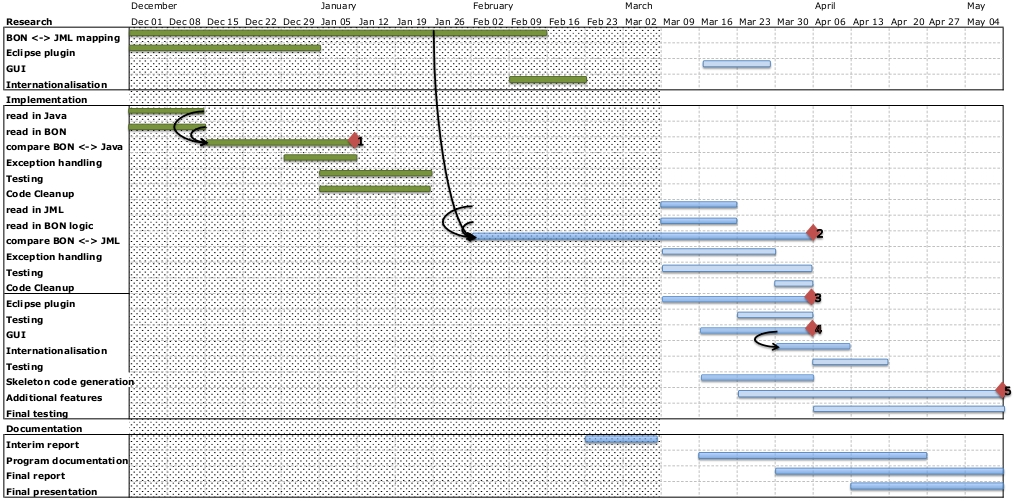
\includegraphics[width = 1\textwidth]{ganttChart_6_march} 
	
\caption{\label{fig:logo} Updated Tasks and Milestones. }
\end{figure} 




%%%% ADD YOUR BIBLIOGRAPHY HERE
\newpage
\begin{thebibliography}{99}

\bibitem{BURDY:2005}Lilian Burdy, Yoonsik Cheon, David Cok, Michael Ernst, Joe Kiniry, Gary T. Leavens, K. Rustan M. Leino, Erik Poll. \emph{An overview of JML tools and applications}. International Journal on Software Tools for Technology Transfer, 7(3):212-232, 2005.

\bibitem{FAIRMICHAEL:2008}Fintan Fairmichael. The BONc project. http://www.kindsoftware.com/products/open source/BONc/.

\bibitem{GOSLING:2005}James Gosling, Bill Joy, Guy Steele, Gilad Bracha. \emph{The Java Language Specification, Third Edition}. 688 pages. ISBN: 0321246780. Addison Wesley, 2005

\bibitem{HORSTMANN:2007}Cay Horstmann \emph{Java Concepts, 5th edition}702 pages. ISBN:0470105550. Wiley, 2007.

\bibitem{LEAVENS:2006}Gary T. Leavens, Albert L. Baker, Clyde Ruby. \emph{Preliminary Design of JML: A Behavioural Interface Specification 
Language for Java}. ACM SIGSOFT Software Engineering Notes, 31(3):1-38, 2006. �http://doi.acm.org/10.1145/1127878.1127884�. Also Iowa State University, Department of Computer Science, TR \#98-06-rev29,  2006. �ftp://ftp.cs.iastate.edu/pub/techreports/TR98-06/TR.pdf�.

\bibitem{LEAVENS:2008}Gary T. Leavens, Erik Poll, Curtis Clifton, Yoonsik Cheon, Clyde Ruby, David Cok, Peter M\"{u}ller, Joseph Kiniry,
Patrice Chalin, Daniel M. Zimmerman \emph{JML Reference Manual}. DRAFT, \$Revision:1.231\$. ftp://ftp.cs.iastate.edu/pub/leavens/JML/jmlrefman.pdf 

\bibitem{MEYER:1992}Bertrand Meyer. \emph{Applying �design by contract�} Computer, 25(10):40�51, 1992. 

\bibitem{MEYER:1997}Bertrand Meyer. \emph{Object-Oriented Software Construction - Second Edition}. 1254 pages. ISBN: 0136291554. Prentice Hall, 1997.

\bibitem{PAIGE:1999} Richard F. Paige, Jonathan S. Ostroff. \emph{A Comparison of the Business Object Notation and the Unified Modeling Language}. Technical Report CS-1999-03. York University, 1999.

\bibitem{PAIGE:2000}Richard F. Paige, Jonathan S. Ostroff. \emph{Precise and Formal Metamodeling with the Business Object
Notation and PVS} Technical Report CS-2000-03, York University, 2000.

\bibitem{RAGHAVAN:2005}Arun D. Raghavan, Gary T. Leavens. \emph{Desugaring JML Method Specifications} Technical Report 00-03e, Computer Science, Iowa State University, 2005.

\bibitem{WALDEN:1995}  Kim Walden, Jean-Marc Nerson. \emph{Seamless Object-Oriented Software Architecture}. 438 pages. ISBN:0130313033. Prentice Hall, 1995. www.bon-method.com.

\bibitem{COK:2008} The OpenJML project. http://www.jmlspecs.org.
\bibitem{EBON:2008}The EBON project. http://ebon.sourceforge.net.





\end{thebibliography}
\label{endpage}

\end{document}

\end{article}
